%!TEX program = xelatex
% 编译顺序: xelatex -> bibtex -> xelatex -> xelatex
% 国家自然科学基金NSFC面上项目申请书正文模板(2023年版)version1.0
% 声明:
% 注意!!!非国家自然科学基金委官方模版!!!由个人根据官方MsWord模版制作。本模版的作者尽力使本模版和官方模版生成的PDF文件视觉效果大致一样,然而,并不保证本模版有用,也不对使用本模版造成的任何直接或间接后果负责。 不得将本模版用于商用或获取经济利益。本模版可以自由修改以满足用户自己的需要。但是如果要传播本模版,则只能传播未经修改的版本。使用本模版意味着同意上述声明。
% 强烈建议自己对照官方MsWord模板确认格式和文字是否一致,尤其是蓝字部分。
% 如有问题,可以发邮件到ryanzz@foxmail.com



\documentclass[12pt,UTF8,AutoFakeBold=2,a4paper]{ctexart} %默认小四号字。允许楷体粗体。
\usepackage[english]{babel} %支持混合语言
\usepackage[dvipsnames]{xcolor}
\usepackage{graphicx} 
\usepackage{amsmath} %更多数学符号
\usepackage{wasysym}
\usepackage[unicode]{hyperref} %提供跳转链接
\usepackage{geometry} %改改尺寸
\usepackage{gbt7714}
\usepackage{natbib}
\setlength{\bibsep}{0.0pt}

%\geometry{left=3.23cm,right=3.23cm,top=2.54cm,bottom=2.54cm}
%latex的页边距比word的视觉效果要大一些,稍微调整一下
%\geometry{left=2.95cm,right=2.95cm,top=2.54cm,bottom=2.54cm}%2020
%\geometry{left=2.95cm,right=2.95cm,top=2.54cm,bottom=2.54cm}
\geometry{left=3.00cm,right=3.07cm,top=2.67cm,bottom=3.27cm}
\pagestyle{empty}
\setcounter{secnumdepth}{-2} %不让那些section和subsection自带标号,标号格式自己掌握
\definecolor{MsBlue}{RGB}{0,112,192} %Ms Word 的蓝色和latex xcolor包预定义的蓝色不一样。通过屏幕取色得到。
% Renaming floats with babel
\addto\captionsenglish{
    \renewcommand{\contentsname}{目录}
    \renewcommand{\listfigurename}{插图目录}
    \renewcommand{\listtablename}{表格}
    %\renewcommand{\refname}{\sihao 参考文献}
    \renewcommand{\refname}{\sihao \kaishu \leftline{参考文献}} %这几个字默认字号稍大,改成四号字,楷书,居左(默认居中) 根据喜好自行修改,官方模板未作要求
    \renewcommand{\abstractname}{摘要}
    \renewcommand{\indexname}{索引}
    \renewcommand{\tablename}{表}
    \renewcommand{\figurename}{图}
    } %把Figure改成‘图’,reference改成‘参考文献’。如此处理是为了避免和babel包冲突。
%定义字号
\newcommand{\chuhao}{\fontsize{42pt}{\baselineskip}\selectfont}
\newcommand{\xiaochuhao}{\fontsize{36pt}{\baselineskip}\selectfont}
\newcommand{\yihao}{\fontsize{26pt}{\baselineskip}\selectfont}
\newcommand{\erhao}{\fontsize{22pt}{\baselineskip}\selectfont}
\newcommand{\xiaoerhao}{\fontsize{18pt}{\baselineskip}\selectfont}
\newcommand{\sanhao}{\fontsize{16pt}{\baselineskip}\selectfont}
\newcommand{\sihao}{\fontsize{14pt}{\baselineskip}\selectfont}
\newcommand{\xiaosihao}{\fontsize{12pt}{\baselineskip}\selectfont}
\newcommand{\wuhao}{\fontsize{10.5pt}{\baselineskip}\selectfont}
\newcommand{\xiaowuhao}{\fontsize{9pt}{\baselineskip}\selectfont}
\newcommand{\liuhao}{\fontsize{7.875pt}{\baselineskip}\selectfont}
\newcommand{\qihao}{\fontsize{5.25pt}{\baselineskip}\selectfont}
%字号对照表
%二号 21pt
%四号 14
%小四 12
%五号 10.5
%设置行距 1.5倍
\renewcommand{\baselinestretch}{1.5}
\XeTeXlinebreaklocale "zh"           % 中文断行

%%%% 正文开始 %%%%
\begin{document}
\begin{center}
{\sanhao \kaishu \bfseries  Hybrid ANNS }
\end{center}

\section{Filtered−DiskANN}
\subsection{1.主要贡献:}
{\sihao \kaishu 本文的主要贡献是两种简单而有效的基于图的过滤 ANNS 算法 - FilteredVamana 和 StitchedVamana,这两种算法均基于Vamana图构建,该图通过创建一个可导航的图结构来高效引导局部“贪心”搜索,使其朝向查询点的最近邻候选者。与现有算法不同,本算法不仅考虑数据集中点的空间位置(即向量坐标),还利用了点的过滤元数据信息。通过结合点之间的几何关系和每个点的标签信息,这两种算法能够构建出更优的图导航结构,从而在近似最近邻搜索中实现更高的效率和准确性。。}

\subsection{2.实现原理:}
\subsubsection{2.1 filteredVamana:}
{\sihao \kaishu filteredVamana图构造属于增量式构建。初始化空图G,为每个过滤标签选择一组起点S,从S出发,对于每个数据点p运行贪婪搜索算法FilteredGreedySearch,从而返回访问顶点集合(集合中所有顶点都具有该过滤标签)。}
{\sihao \kaishu 当搜索过程中某个点的出度超过规定范围,使用剪枝算法FilteredRobustPrune修剪。 }


\subsubsection{2.2 stitchedVamana:}
{\sihao \kaishu 如图\ref{fig:1}所示,对于每一个过滤标签f,构建对应的vamana图,然后将这些图合并(边集取并)成一个图G,G与filteredVamana所构建的图兼容。它只能在提前知道点集的情况下使用,无法实现增量式构建。}
\begin{figure}[!th]
\begin{center}
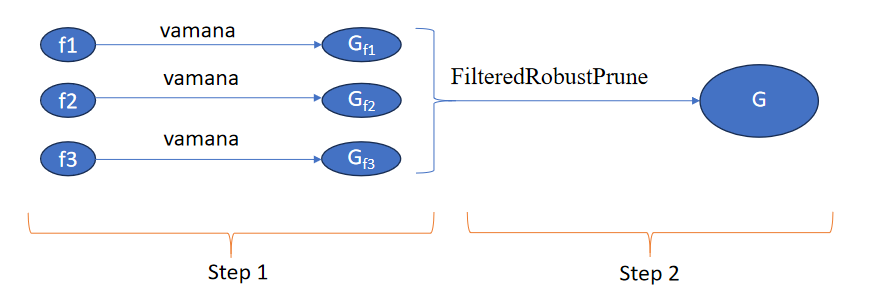
\includegraphics[width=5in]{stitchedvamana.png}
\caption{{\kaishu stitchedVamana实现原理}}
\label{fig:1}
\end{center}
\end{figure}
\subsubsection{2.3 比较:}
{\sihao \kaishu filteredVamana:能够通过点插入实现动态索引增长。稳健性更好,索引构建时间更快。}

{\sihao \kaishu stitchedVamana:不能实现动态索引增长。QPS和召回率表现更好。}


\subsection{3.优势:}
{\sihao \kaishu (1)索引构建时,不仅考虑点的向量坐标,也考虑过滤标签,真正将过滤信息融合在图索引构建中。}

{\sihao \kaishu (2)filteredVamana支持在SSD上查询,节约内存。}

{\sihao \kaishu (3)稀疏属性不受影响。}

{\sihao \kaishu (4)filteredVamana支持动态插入。}

\subsection{4.缺陷:}
{\sihao \kaishu 本方法无法支持任意复杂的过滤条件,而只能支持简单枚举型条件,可以支持多个条件的OR,但是不支持AND。专注于单个过滤器与查询相关联的情况。}



{\section{NHQ 算法}}
{\subsection{ 1.1 概述}}
本文通过提出融合距离来实现混合索引,以便在查询过程中同时支持特征向量和属性约束,而不是像传统方法那样将查询分解为独立的向量相似性搜索和属性过滤两个子任务;还提出了两种新颖的可导航近邻图,它们采用优化的边选择和路由策略,从而显著提高了混合查询的整体性能。




{\subsection{1.2具体实现}}
NHQ 提出了融合距离来实现原生的混合查询框架,融合距离定义如~\ref{eq:merged_distance}所示,其中的$\chi\left(\ell\left(e_i\right), \ell\left(e_j\right)\right)$表示标签距离,用于描述两个对象之间的标签是否相同,通过计算其相同的属性数来获得,如~\ref{eq:lable_dist}和~\ref{eq:lable_dist2}所示.


\begin{equation}
\chi\left(\ell\left(e_i\right), \ell\left(e_j\right)\right)=\sum_{k=0}^{m-1} \phi\left(\ell\left(e_i\right)^k, \ell\left(e_j\right)^k\right)
    \label{eq:lable_dist}
\end{equation}
\begin{equation}
\phi\left(\ell\left(e_i\right)^k, \ell\left(e_j\right)^k\right)= \begin{cases}0, & \ell\left(e_i\right)^k=\ell\left(e_j\right)^k \\ 1, & \ell\left(e_i\right)^k \neq \ell\left(e_j\right)^k\end{cases}
    \label{eq:lable_dist2}
\end{equation}

\begin{equation}
\Gamma\left(e_i, e_j\right)=\omega_\nu \cdot \delta\left(\nu\left(e_i\right), \nu\left(e_j\right)\right)+\omega_{\ell} \cdot \chi\left(\ell\left(e_i\right), \ell\left(e_j\right)\right)
\label{eq:merged_distance}
\end{equation}

在公式 $1-2$ 中,$m$ 是 $\ell\left(e_i\right)$ 的维度数量,$\ell\left(e_i\right)^k$ 表示 $\ell\left(e_i\right)$ 在第 $k$ 个维度上的取值。$\chi\left(\ell\left(e_i\right), \ell\left(e_j\right)\right)$ 越小,$\ell\left(e_i\right)$ 与 $\ell\left(e_j\right)$ 的相似度越高。

通过融合距离的定义,NHQ算法可以在索引构建时直接考虑向量相似度和标签相似度,构建出PG混合索引,直接在该索引上进行混合查询,而不需要额外的计算和内存开销。并且,该框架对PG图支持友好,可以将融合距离用于其他PG图,从而达到混合查询的效果。

除了原生的混合查询框架,文中还提出了新的边缘选择策略以及路由策略来实现可导航近邻图。由于PG图直接选取最近的点作为邻居可能会导致邻居聚集在一起,搜索时探索区域有限。文中提出了新的边缘选择策略来解决邻居分布聚集的问题,在选择邻居时,首先选取最近的,之后通过远点和邻居节点的垂直平分线分割出原点所在区域,以及原点和邻居节点的距离为半径画的圆外的区域,两个区域的交集定义为着陆区,新的邻居必须从着陆区选取,循环选取邻居,从而实现邻居分布均匀。如图\ref{fig:edge}所示。
\begin{figure}[h] % 这里的 [h] 表示将图片放在当前位置(here)
    \centering % 使图片居中
    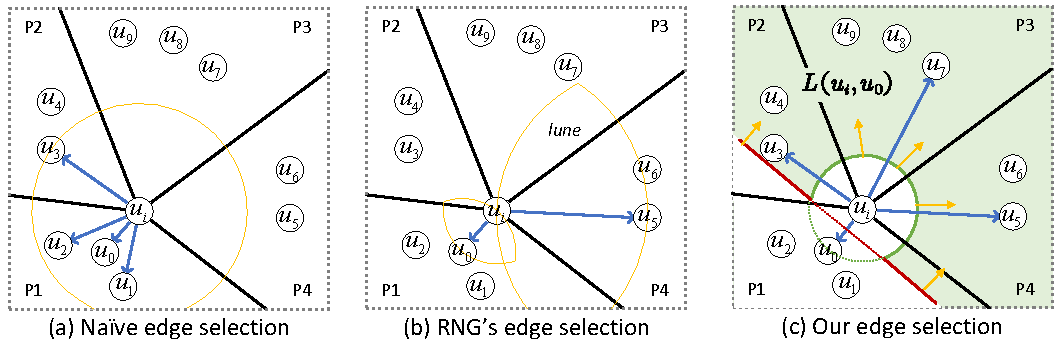
\includegraphics[width=1\textwidth]{edge_selection.pdf} % 调整图片的宽度,并插入图片文件
    \caption{边选择策略}
    \label{fig:edge} % 设置图片的标签,以便引用
\end{figure}

边选择策略使得邻居分布均匀,随机两阶段路由策略则加速搜索过程。文中提出的两阶段路由策略在最开始时,随机选取部分点进行探索,当靠近目标点之后,再进行贪心策略进行搜索,从而减少访问点的次数以及计算量。



{\subsection{1.3优势}}
目前的混合查询方法基本采用分别维护两个索引的方式来进行混合查询,在查询时先进行向量相似化搜索,之后再进行属性过滤,或者顺序相反;但同时维护两个索引的方法,会产生不必要的内存花销和计算,查询结果依赖于两个结果的合并,可能不精确,对现有的PG图支持也不是很友好,没能利用PG图的优势。NHQ通过使用其融合距离,在构建索引时同时考虑向量相似度和标签,只用构建一个索引即可完成混合查询,且兼容大部分的PG图,提出了原生的混合查询框架,并且查询时,尽可能的满足多标签,而不是只满足其中一个,有着不错的效果。


{\subsection{1.4缺陷}}
论文提出的融合距离,实现了原生的混合查询框架,适用于大部分PG图,同时正对PG图,又提出了新的边缘选择策略以及路由策略,以此来加快搜索,二者结合,再最终的实验表现上有着很好的结果。但NHQ考虑的设置是每个数据点实际上只有一个相关的过滤器标签,即一一类标签下,各标签点的集合不相交,这种情况可以通过每个过滤器的单独标准 ANNS 索引来处理。此外,这种技术在缩放到每个点多个过滤器/标签时可能无效,而不显著影响召回。如果索引中的一个点有三个过滤器标签,而查询只有一个,则其他两个标签中的距离会对总的距离产生不利影响。





% {\sihao \kaishu 参照以下提纲撰写,要求内容翔实、清晰,层次分明,标题突出。{\color{MsBlue} \bfseries 请勿删除或改动下述提纲标题及括号中的文字。}}
% \vskip -5mm
% {\color{MsBlue} \subsection{\sihao \kaishu \quad \ (一)立项依据与研究内容(建议8000字以下): }}

% {\sihao \kaishu \color{MsBlue} 1.{\bfseries 项目的立项依据}(研究意义、国内外研究现状及发展动态分析,需结合科学研究发展趋势来论述科学意义;或结合国民经济和社会发展中迫切需要解决的关键科技问题来论述其应用前景。附主要参考文献目录);}

% 对于习惯用 \LaTeX 写文档的老师和同学们,一个写基金申请书的模版可能有参考作用。因此我做了这个{\bfseries \color{Bittersweet} 面上项目}申请书正文部分模版,供参考。

% 2023-01-20: 根据2023年面上项目申请书正文的官方MsWord模板,对本模板的字号和少量蓝色文字做了更新。

% 2023-01-29\&02-01: 根据几位老师的建议,对section的缩进,“参考文献”四个字的大小、字体和居左等做了调整。官方模板中阿拉伯数字不加粗,因此也做了相应的调整。



% \begin{figure}[!th]
% \begin{center}
% 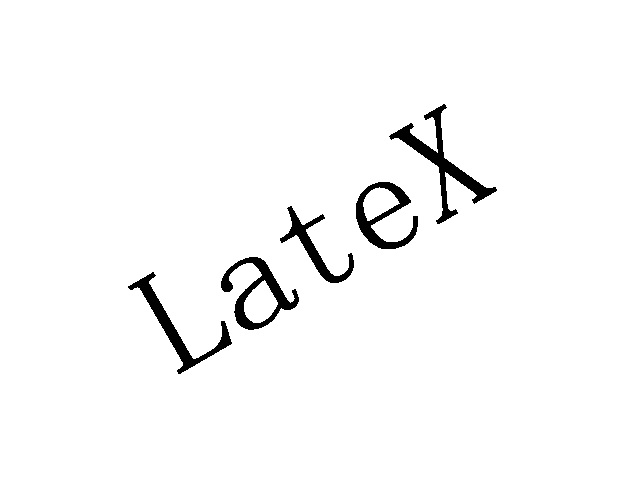
\includegraphics[width=2in]{fig-example.eps}
% \caption{{\kaishu 插图可以使用EPS、PNG、JPG等格式。}}
% \label{fig:example}
% \end{center}
% \end{figure}

% 2023-02-06: 根据@Readon的commits,做了如下修改:1. 更正了一处蓝字部分:``(三)其他需要说明的问题'' $\rightarrow$ ``(三)其他需要说明的情况'' 。这个非常重要!2. 设置 AutoFakeBold=3,这样楷体粗体稍微细一点,和官方模板更加接近。3. 调整了页面空白的宽度,大家可以自行微调。作为\LaTeX 菜鸟,非常感谢Readon的专业建议!更多专业的修改请见\url{https://github.com/Readon/NSFC-application-template-latex}

% 2023-12-04:一转眼2024年的申请又要开始了。主要做了两点修改:1. 把图的caption字体调整为楷体。2. 设置AutoFakeBold=2,个人感觉这样和MsWord模板中的粗体更接近一点。等官方模板更新之后我再做相应更新。

% 2023-12-30:改用GB/T 7714 (numerical) 样式以支持中文文献。 这样做的另外一个优点是该包兼容natbib,修改参考文献的行距也比较方便,这里也缩短了一些。如有需要,也可以切换回ieeetrNSFC。



% \vskip 2mm
% \subsubsection{1.1 声明}
% {\bfseries \color{red} 注意!!!非国家自然科学基金委官方模版!!!}由个人根据官方MsWord模版制作。本模版的作者尽力使本模版和官方模版生成的PDF文件视觉效果大致一样,然而,并不保证本模版有用,也不对使用本模版造成的任何直接或间接后果负责。 不得将本模版用于商用或获取经济利益。本模版可以自由修改以满足用户自己的需要。但是如果要传播本模版,则只能传播未经修改的版本。使用本模版意味着同意上述声明。

% 祝大家基金申请顺利!如有问题,请发送邮件到 \href{mailto:ryanzz@foxmail.com}{ryanzz@foxmail.com}。中了基金的也欢迎反馈。$\smiley$

% \subsubsection{1.2 使用说明}\label{sss:instruction}

% \begin{enumerate}
% \item 编译环境:推荐使用跨平台编译器texlive2017以后的版本,编译顺序为:xelatex+bibtex+xelatex(x2)。windows用户可以用命令行运行批处理文件getpdf.bat,linux用户可以运行runpdf。
% \item 本模版力求简单,语句自身说明问题(self explanatory)。几乎只需要修改本tex文件即可满足排版需求,没有sty cls 等文件。用户掌握最基本的\LaTeX 语句即可操作,其余的可以用搜索引擎较容易地获得。
% \item 参考文献样式:从2023.12.30版本开始,采用GB/T 7714 (numerical) 样式以支持中文文献,这样做的另外一个优点是该包兼容natbib,修改参考文献的行距也比较方便,缩短了一些。如有需要,也可以切换回ieeetrNSFC。
% \end{enumerate}

% \subsubsection{1.3 图、公式和参考文献的引用示例}
% 尽管不大可能会用到像下面这样简单的公式:
% \begin{equation}
% \label{eq:ex}
% \sqrt[15]{a}=\frac{1}{2},
% \end{equation}
% 我们还是用公式(\ref{eq:ex})举个数学公式的例子。同时,我们也不大可能会用到一个长得很像\LaTeX 的图,但是还是引用一下图\ref{fig:example}。图\ref{fig:example}并没有告诉我们关于Jinkela\cite{John1997,Smith1900}的任何信息,也没有透露它的产地\cite{Piter1992,grif1998}。尽管如此,最近的研究表明,Feizhou非常需要Jinkela\cite{John1997}。


% %从2023.12.30版本开始,采用GB/T 7714 (numerical) 样式以支持中文文献,这样做的另外一个优点是该包兼容natbib,修改参考文献的行距也比较方便,缩短了一些。如有需要,也可以切换回之前版本用的ieeetrNSFC
% %\newpage
% %\bibliographystyle{ieeetrNSFC}
% \bibliographystyle{gbt7714-numerical}
% \bibliography{myexample}
% \newpage

% {\sihao \color{MsBlue} \kaishu 2. {\bfseries 项目的研究内容、研究目标,以及拟解决的关键科学问题}(此部分为重点阐述内容);}

% 本项目的{\bfseries 研究目标}是获得申请面上项目的\LaTeX 模版。

% 拟解决的{\bfseries 关键问题}包括:

% \begin{itemize}
% \item 中文的处理。
% \item 参考文献\cite{John1997,Smith1900,Piter1992}的样式。
% \item 官方word模版中蓝色的获得。
% \end{itemize}




% {\sihao \color{MsBlue} \kaishu 3.{\bfseries 拟采取的研究方案及可行性分析} (包括研究方法、技术路线、实验手段、关键技术等说明);}

% 详见1.2使用说明。

% {\sihao \color{MsBlue} \kaishu 4.{\bfseries 本项目的特色与创新之处;}}

% 本模版修改自由度很高,可以按照用户自己的需求修改而不要求用户具有很多\LaTeX 技巧。


% {\sihao \color{MsBlue} \kaishu 5.{\bfseries 年度研究计划及预期研究结果}(包括拟组织的重要学术交流活动、国际合作与交流计划等)。}

% 拟组织研讨会1次,将这个模版广而告之。但是目前还没有经费。

% \vskip -5mm %可以通过类似的命令微调行距以使得排版美观

% {\color{MsBlue} \subsection{\sihao \kaishu \quad \ (二)研究基础与工作条件 }}

% {\sihao \color{MsBlue} \kaishu 1.{\bfseries 研究基础}(与本项目相关的研究工作积累和已取得的研究工作成绩);}

% 申请人用\LaTeX 写过几篇文章,包括自己的博士论文。

% {\sihao \color{MsBlue} \kaishu 2.{\bfseries 工作条件}(包括已具备的实验条件,尚缺少的实验条件和拟解决的途径,包括利用国家实验室、国家重点实验室和部门重点实验室等研究基地的计划与落实情况);}

% 申请人课题组具有可以编译 \LaTeX 的计算机,可以成功编译此模版。

% {\sihao \color{MsBlue} \kaishu 3.{\bfseries 正在承担的与本项目相关的科研项目情况}(申请人和主要参与者正在承担的与本项目相关的科研项目情况,包括国家自然科学基金的项目和国家其他科技计划项目,要注明项目的资助机构、项目类别、批准号、项目名称、获资助金额、起止年月、与本项目的关系及负责的内容等);}

% 无。

% {\sihao \color{MsBlue} \kaishu 4.{\bfseries 完成国家自然科学基金项目情况}(对申请人负责的前一个已资助期满的科学基金项目(项目名称及批准号)完成情况、后续研究进展及与本申请项目的关系加以详细说明。另附该项目的研究工作总结摘要(限500字)和相关成果详细目录)。}

% 不告诉你。

% {\color{MsBlue} \subsection{\sihao \kaishu \quad \ (三)其他需要说明的情况 }}

% {\sihao \color{MsBlue} \kaishu 1. 申请人同年申请不同类型的国家自然科学基金项目情况(列明同年申请的其他项目的项目类型、项目名称信息,并说明与本项目之间的区别与联系)。 }

% 无。

% {\sihao \color{MsBlue} \kaishu 2. 具有高级专业技术职务(职称)的申请人或者主要参与者是否存在同年申请或者参与申请国家自然科学基金项目的单位不一致的情况;如存在上述情况,列明所涉及人员的姓名,申请或参与申请的其他项目的项目类型、项目名称、单位名称、上述人员在该项目中是申请人还是参与者,并说明单位不一致原因。}

% 无。

% {\sihao \color{MsBlue} \kaishu 3. 具有高级专业技术职务(职称)的申请人或者主要参与者是否存在与正在承担的国家自然科学基金项目的单位不一致的情况;如存在上述情况,列明所涉及人员的姓名,正在承担项目的批准号、项目类型、项目名称、单位名称、起止年月,并说明单位不一致原因。}

% 无。

% {\sihao \color{MsBlue} \kaishu 4. 其他。}

% 无。
\end{document}


